\documentclass{standalone}
\usepackage{tikz}
\usepackage{verbatim}
\usetikzlibrary{positioning}
\begin{document}
\pagestyle{empty}
  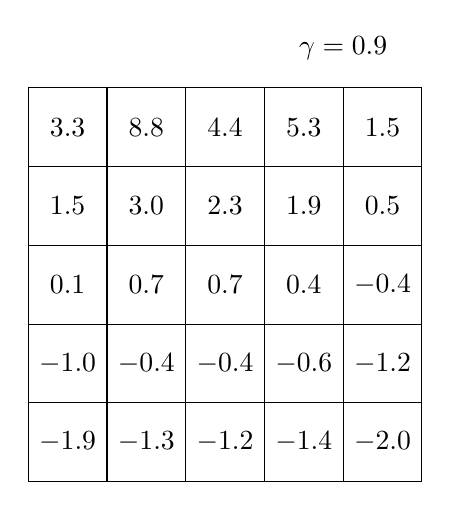
\begin{tikzpicture}
    \draw[step=1.0,black,thin] (0,0) grid (5, 5);
    % Bottom row
    \node at (0.5, 0.5) {$-1.9$};
    \node at (1.5, 0.5) {$-1.3$};
    \node at (2.5, 0.5) {$-1.2$};
    \node at (3.5, 0.5) {$-1.4$};
    \node at (4.5, 0.5) {$-2.0$};
    % Second to last row from bottom
    \node at (0.5, 1.5) {$-1.0$};
    \node at (1.5, 1.5) {$-0.4$};
    \node at (2.5, 1.5) {$-0.4$};
    \node at (3.5, 1.5) {$-0.6$};
    \node at (4.5, 1.5) {$-1.2$};
    % Middle row
    \node at (0.5, 2.5) {$0.1$};
    \node at (1.5, 2.5) {$0.7$};
    \node at (2.5, 2.5) {$0.7$};
    \node at (3.5, 2.5) {$0.4$};
    \node at (4.5, 2.5) {$-0.4$};
    % Second row from top
    \node at (0.5, 3.5) {$1.5$};
    \node at (1.5, 3.5) {$3.0$};
    \node at (2.5, 3.5) {$2.3$};
    \node at (3.5, 3.5) {$1.9$};
    \node at (4.5, 3.5) {$0.5$};
    % Top row
    \node at (0.5, 4.5) {$3.3$};
    \node at (1.5, 4.5) {$8.8$};
    \node at (2.5, 4.5) {$4.4$};
    \node at (3.5, 4.5) {$5.3$};
    \node at (4.5, 4.5) {$1.5$};
    % Gamma factor for clarity.
    \node at (4, 5.5) {$\gamma = 0.9$};
  \end{tikzpicture}
\end{document}